\documentclass[journal]{IEEEtran}
\usepackage{cite}




 \usepackage[pdftex]{graphicx}



\begin{document}
\title{Effective Tumor Classification Exploiting Volumetric Image Analysis}
\author{Ashley J. Robinson}

% The paper headers
\markboth{Southampton University, Department of Electronics and Computer Science, Independent Research Review.}%
{Robinson: Effective Tumor Classification Exploiting Volumetric Image Analysis}

\maketitle


\begin{abstract}

\dots

\end{abstract}







\begin{IEEEkeywords}
Tumor, Classification
\end{IEEEkeywords}



\IEEEpeerreviewmaketitle







\section{Introduction}
\IEEEPARstart{T}{his} research review covers the use of volumetric image analysis in medicine to accurately classify tumors. 
The problem is to be approached by considering only the general case where no specific area of the human body is considered.
Rather than trying to classify lung or brain tumors individually the goal is to consider what tumors have in common and given an entire image of a human body is it possible to classify tumors in any given section?
The motivation behind this is to make the most of medical scanning.
Dosages of radiation, cost and simply the time required are all reasons to reduce the number of scans needed, making the most of any data gathered is a constructive method of scan frequency reduction.
The objective is to provide a recommendation for a system to be implemented such that a medical practitioner could use it as a tool for diagnosis.  

The architecture in Fig.~\ref{fig:Proposed} is a simplistic view of the system to be recommended; inspired by those discussed in ~\cite{ahmed2011efficacy,kumar2011classification,sachdeva2011multiclass}.
A chain of stages leads from raw data gathered from the patient to a diagnosis from a classification algorithm.
A confidence sub-block enables the domain expert to view the performance of the entire system without knowing the intricacies of operation; this requires processing to be explained with respect to their domain.
Raw data is captured from the patient and passed to system for pre-processing then feature extraction.
Input patterns are produced from volumetric feature extraction dependent on a pre-determined list of known useful features. 
Feature reduction and normalisation is then used frame the data as such to make the most of the classification algorithm used to provide support for diagnosis.

\begin{figure}[!htb]
   \centering
   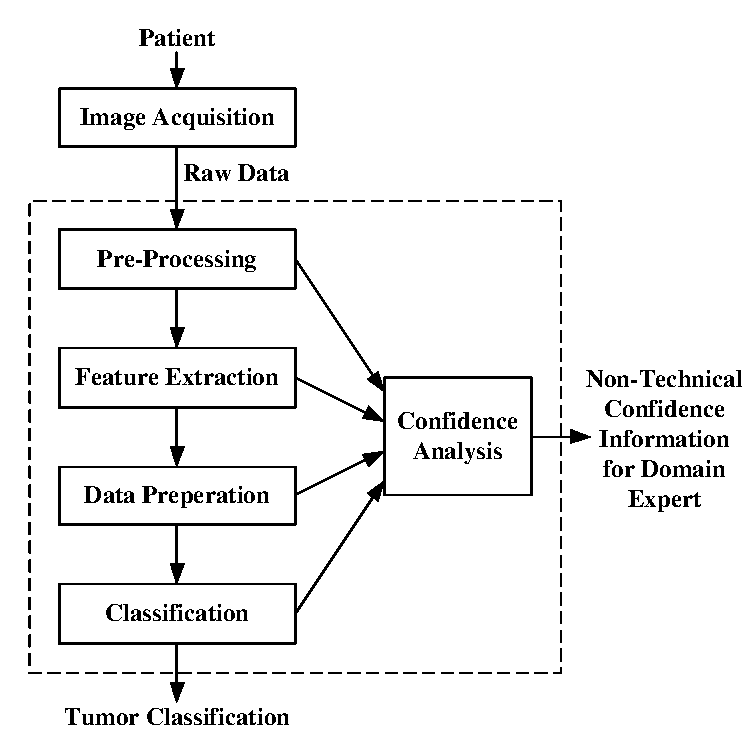
\includegraphics[width = 0.35\textwidth]{Figures/Proposed.pdf}
   \label{fig:Proposed}
   \caption{Proposed system architecture.}
\end{figure}











\section{Image Acquisition}
\label{sec:image}

A standard X-ray will produce a shadow cast by the absence of light due to bone or other material in the human body.
This uses a single source and substrate to capture the image.
Taking multiple images from many different angles gathers more information and a 3D image can be made by stitching these together.
Fig.~\ref{fig:ct} describes the physical process of gathering data to be used in Computed Tomography (CT).
A ring allows images to be capture from 360$^{\circ}$ in a single plane then by moving in the orthogonal plane, in Fig.~\ref{fig:ct} through the paper, a full volumetric image of the patient can be made. 

\begin{figure}[!htb]
   \centering
   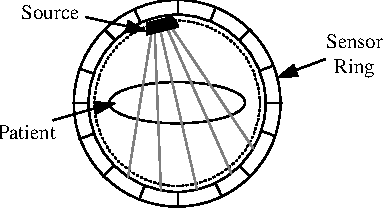
\includegraphics[width = 0.15\textwidth]{Figures/CT.pdf}
   \label{fig:ct}
   \caption{Acquiring data from Computed Tomography. Adapted from~\cite{kayvan2006biomedical}.}
\end{figure}

Any method of non-invasive image capturing in 2D can therefore by expanded to work in 3D by using the CT principle.
Different methods have trade offs such as radiation dosages and resolution.
Ultrasound is a method of image acquisition with the advantage of small processing overhead allowing an internal organs to be view in real-time. 
It can be used for CT but higher resolution methods are favoured such as X-ray and Magnetic Resonance Imaging.

There are also other non-intrusive methods that don't use electromagnetic or ultrasonic waves.
Hand palpitation is a common technique used by medical practitioners to gain an impression of abnormalities near the surface of the human body. 
Electromechanical apparatus employing the same technique can be used transfer the dimension of a growth to a volumetric image~\cite{liu09haptic,wellman1997modeling}.  
This offers far less data for analysis.

Data is typically stored as a series of grayscale 2D images which are slices of the scan.
The image viewer will build 3D images as and when required using these slices.
The common medical standard for these images is DICOM which holds the relationships between slices and also patient information~\cite{dicom11nema}.
Viewing the data naturally proves problematic because it is 3D data shown in an isometric fashion on a 2D screen.
Viewing software provides interactive images as shown in Fig.~\ref{fig:3d} which allows the user to move three slices to concentrate on corner on specific points.

\begin{figure}[!htb]
   \centering
   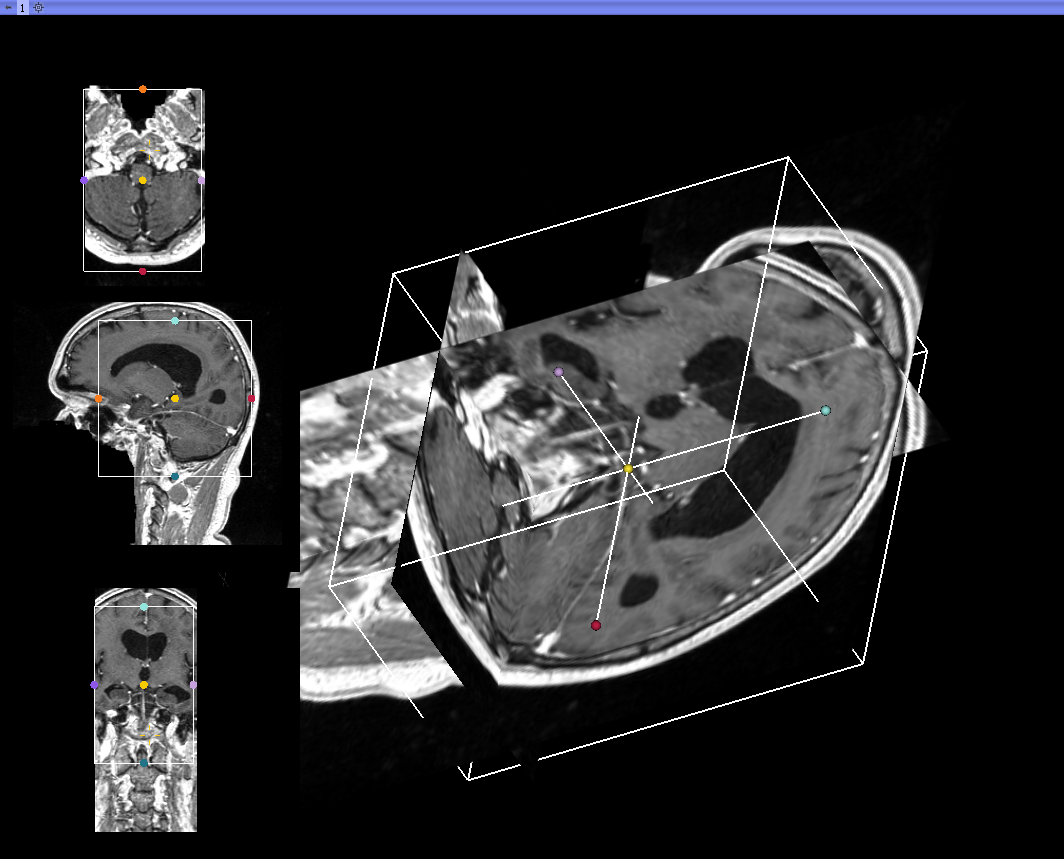
\includegraphics[width = 0.4\textwidth]{Figures/3Dview.png}
   \label{fig:3d}
   \caption{An MRI scan of a healthy brain taken from~\cite{cia} and rendered by~\cite{slicer}.}
\end{figure}

The analogue of a pixel (picture element) in 2D image is called a voxel (volumetric element) in a 3D image.
This is exactly ther same idea but with a extra dimension to form a cube~\cite{lohmann1998volumetric}.
They can be considered cubes but also points which may make visualisation and processing easier to understand.







\section{Pre-processing}
\label{sec:pre}

The provided raw data needs to be converted from the format delivered by the acquisition technology to a three dimensional matrix ready for generic processing.
Removal of watermarking, which may have been inserted for human review, should also be removed at this stage. 
This is trivial in theory but requires a database of artifacts or manual review to accomplish.

Filters can be used to enhance the quility of images.
These are split two catagroies, linear and non-linear~\cite{lohmann1998volumetric}.
Linear filtering is achieved by using a mask to weight each voxel the surrounding voxels.
This is done with a weighted mask which is applied to image in path which covers all regions.


\subsection{Histogram Operations}

An image histogram is a simple yet powerful tool which is a mapping from the image to 2D plot of the frequency of each voxel.
This contains information on the type of material seen in the image and how much of that material us used to form the entire image.
Operations can also be performed on the image using this information to improve the contrast.

\begin{figure}[!htb]
   \centering
   \includegraphics[width = 0.4\textwidth]{Figures/Histogram.png}
   \label{fig:histogram}
   \caption{The histogram of the image shown in Fig.~\ref{fig:3d}}
\end{figure}




\subsection{Spatial Filtering}

\subsection{Frequency Filtering}
%Real-time methods of speckle reduction are used to improve the quilitiy of unltrasound images~\cite{mustafa95speckle}.






\section{Feature Selection}
\label{sec:selection}
Before features can be extracted from a image it must be clear what features will be useful to a classification algorithm.
Reducing dimensionality through feature reduction can often prove more effective then lower dimensional projection methods; discussed in Section~\ref{sec:reduce}.
The recommendation of feature selection can come from domain knowledge or convergence on a subset that will provided a sufficiently low training error using an iterative tuning algorithm~\cite{bu07feature,li10tumor}.
A combination of both suits this purpose where domain knowledge may over recommend features and a machine learning approach can prune as required for the subset.  



\section{Feature Extraction}
\label{sec:extraction}





\section{Dimensionaility Reduction}
\label{sec:reduce}




\section{Classification}
\label{sec:class}




\section{Conclusion}
\label{sec:conclusion}

It is clear that this tool can't be used as a hard and fast method of tumor diagnosis but instead as a valuable tool for image reviewers.
Software packages designed for medical image review, such as~\cite{slicer}, have bidirectional interfaces to custom extensions.
Implementing this system as an extension would remove many overheads required in data handling but reduce the scope for optimisation.
The feedback from the entire process would be a checklist which the user must manually review and waive if incorrectly identified. 


\bibliographystyle{ieeetran}
\bibliography{references}

\end{document}


